\section{Introduction}
\label{sec:introduction}
\subsection{Background}
\paragraph{}As the world’s industries push the boundaries of optimization and efficiency, the exponential increase in computational ability and technology The automation of “higher-level” tasks that require human intellect is now possible. This headway brings unmanned autonomous vessels within the Maritime Industry closer to mass production. The practicality of autonomous vessels can only be achieved with constant awareness of the performance and operating state of machinery in the engine room (CBM).  Observations of industry practices display that industry experience in reliability is heavily based on trial-and-error test procedures. 

\paragraph{}Most of the reliability research in industry still focuses on two distinct periods of the product life. The warranty period, where most of the failures are due to product malfunctions or quality related problems, and, wear-out period, where the failures are due excessive wear and use(1). Using sensors and logging software the condition of equipment is assessed as  frequently as needed, enabling efficient analysis of data that facilitates planning of predictive maintenance on-board vessels. 
\paragraph{}The  electric motor is the most used device for conversion from electric to mechanical energy and is used for electric propulsion,  powering thrusters for station keeping, and different on-board equipment on hundreds of ships. Typically, 80-90 percent of the load installations will be electric motors.\cite{noauthor_all_2019}
\paragraph{}Smart organizations know they can no longer afford to see maintenance as just an expense. Rather, maintenance must be integrated within the business cycle in order to guarantee predictability, growth and increase the overall quality of operations. Moving from a regime of scheduled rule-based maintenance via on-condition maintenance and ultimately to a data-driven risk-based regime can lead to more accurate and timely maintenance tasks. This smarter view of maintenance allows for achieving many practical advantages leading to lower costs and increased safety and availability of ship
systems.\cite{knutsen_beyond_2014}
\begin{figure}
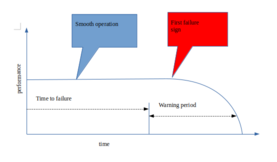
\includegraphics{Figures/figure_1}
\caption{Fuel Cell Structure
\cite{pukrushpan_modeling_2003}}
\end{figure}

\paragraph{}Making  failure predictions and determination of remaining useful life (RUL), realizes significant benefits not limited to: work=style reforms, reduction in crew workload in that monitoring is done autonomously, improved safety from preventing accidents before they happen, and ensuring efficient optimal operation.
\cite{gaeid_diagnosis_2010}
In future more equipment will be added in a modular manner to realize better optimal performance.

\paragraph{}There are several types of fuel cells, each using a different chemistry. The common types of fuel cells are:
\begin{itemize}
\item Polymer electrolyte fuel cells
\item Direct methanol fuel cells
\item Alkaline fuel cells
\item Phosphoric acid fuel cells
\item Solid oxide fuel cells
\item Reversible fuel cells
\item Molten carbonate fuel cells
\end{itemize}
\paragraph{}Polymer electrolyte fuel cells and alkaline fuel cells were the commonly used fuel cells for space missions. Development of fuel cells for commercial activities started in 2007, with an interest to develop fuel cells for automobile applications. The Polymer Electrolyte membrane (PEM) fuel cell is commonly used to power vehicles. Currently, the Polymer Electrolyte Membrane (PEM) Fuel Cells (also known as Proton Exchange Membrane Fuel Cells) are considered by many to be in a relatively more developed stage for ground vehicle applications. PEM Fuel Cells have high power density, solid electrolyte, long cell and stack life, as well as low corrosion. They have greater efficiency when compared to heat engines and their use in modular electricity generation and propulsion of electric vehicles is promising \cite{holze_supramanian_2007}. This proposal will focus on the design and development of a control system for a Proton Exchange Membrane Fuel Cell (PEMFC).

\subsection{Basic Operation Principle }
\begin{figure}[!h]
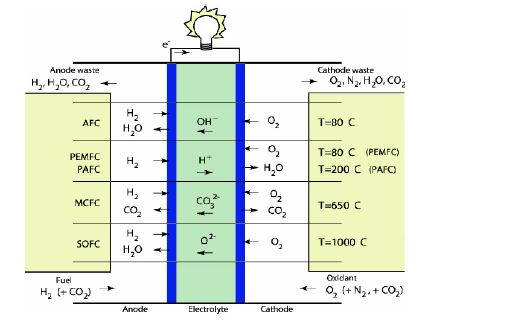
\includegraphics{Figures/Figure1}
\caption{Fuel cell types and their respective operating temperatures
\cite{stefanopoulou_mechatronics_nodate}}
\end{figure}
\begin{figure}[!h]
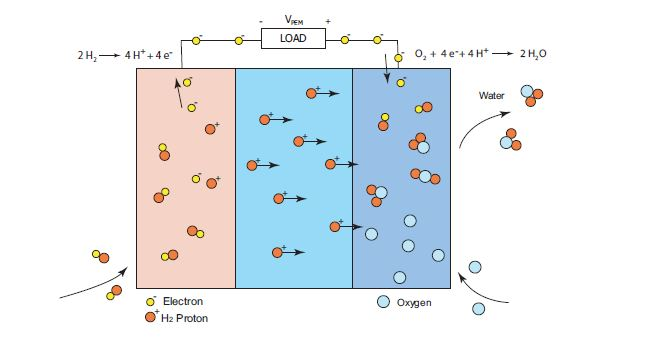
\includegraphics{Figures/Figure2}
\caption{Fuel Cell Reactions
\cite{pukrushpan_modeling_2003}}
\end{figure}
\paragraph{}Fuel cells convert chemical energy sources directly to electricity. A fuel cell consists of an electrolyte sandwiched between two electrodes. The electrolyte has a special property which allows protons to pass through while blocking electrons. Hydrogen gas passes over one electrode, i.e. an anode, and with the help of a catalyst, separates into electrons and hydrogen protons.
\begin{equation}
$$2H_{2}\rightarrow 4H^{+} + 4e^{-}$$
\end{equation}
\paragraph{}The protons flow to the other cathode through the electrolyte while the electrons flow through an external circuit, thus creating electricity. The hydrogen protons and electrons combine with oxygen flow through the cathode, and produce water.
\begin{equation}
$$O_{2}+ 4H_{2} + 4e^{-} \rightarrow 2H_{2}O $$
\end{equation}
\paragraph{}The overall reaction of the fuel cell is given by:
\begin{equation}
$$2H_{2}+ O_{2} \rightarrow 2H_{2}O $$
\end{equation}

\subsection{Problem statement}
\paragraph{} Out of 880 accidental errors in ship related incidents 62% are attributed to human failure; of this, 22% are eq% shipboard related operations1. The adversuipment failure and 72e and often negative impacts of these cases are spread throughout the financial, safety and environmental aspects of the shipping industry. 
Engine room failures are caused by a majority of three ways, either by:  Natural mechanical failure, Electrical failure of components and whole systems, Human negligence, and poor competency in engine room procedures, Inaccurate diagnosis, and sub-par prevention measures.
\paragraph{}These accidents are more notably recognized when they result in internationally felt effects such as oil spills damaging large swathes of marine ecosystems or when loss of life of crew members is realised. But with greater significance but less spoken of - the loss of millions in profits in maintenance and shipping costs incurred to the vessel's owner that would otherwise have been used more productively.

\paragraph{}While it is impractical to try and eliminate accidents in the engine room,this design proposal seeks to provide a solution to improving efficiency and mitigating downtime by implementing strategies to reduce human through the automation of engine room condition monitoring\cite{stefanopoulou_mechatronics_nodate}.
\subsection{Objectives}
\subsubsection{Main Objectives}
\begin{enumerate}
\item To develop monitor the health of ship motors improving reliability and preventing downtime in ships.

\end{enumerate}
\subsubsection{Specific Objectives}
\begin{enumerate}
\item To develop a predictive maintenance algorithm for electric motors in ships.
\item To model a modular framework onto which various equipment will be added to achieve predictive maintenance in the entire ship's engine room. 
\item To design a product that has seamless integration on multiple motors
\end{enumerate}
\subsection{Justification of the study}
\paragraph{}Electric motors serve as a critical component for any facility. However, electric motors can be prone to any number of issues that lead to motor faults and failures. Failures disrupt business operations, decrease productivity, and adversely impact a company’s bottom line.
\paragraph{}Motor inspection processes have shifted from manual scrutiny to semi automated and fully-automated inspection. This will replace the time consuming task of manual review, significantly increasing productivity while preventing missed inspection as well as errors.
Traditionally maintenance involves routine inspection and repair done manually. This cannot completely prevent the risk of machine downtime and will also result in the unnecessary early replacement of usable parts.
\cite{ritchie_comparative_2000}
\paragraph{}The purpose of this project is to alert about problems occurring in the motor and trying to mitigate the risk of unexpected failure. A well planned predictive maintenance is the key to long life operation of motors. In ships unexpected failure causes downtime which deeply eats into profits.The traditional approach is to repair and replace equipment after a period of time but this cannot prevent downtime due to malfunctions, which put a halt to operations and incur massive losses. Advanced monitoring is implemented on parts that are about to break down and can be discovered in advance to accurately determine the time for repair and risk of unexpected shutdown can be prevented.
 \cite{xu_hierarchical_2010}
\paragraph{}  Although Reactive and preventive maintenance will always have a part in operations,Predictive maintenance is the next big step forward in the evolution of asset management. In fact, the ability to connect assets and feed information into a central system gives organizations the power to turn data into powerful insights and automatically take corrective, preventive or predictive action.